% Options for packages loaded elsewhere
\PassOptionsToPackage{unicode}{hyperref}
\PassOptionsToPackage{hyphens}{url}
\PassOptionsToPackage{dvipsnames,svgnames,x11names}{xcolor}
%
\documentclass[
  letterpaper,
  DIV=11,
  numbers=noendperiod]{scrreprt}
\usepackage{amsmath,amssymb}
\usepackage{lmodern}
\usepackage{iftex}
\ifPDFTeX
  \usepackage[T1]{fontenc}
  \usepackage[utf8]{inputenc}
  \usepackage{textcomp} % provide euro and other symbols
\else % if luatex or xetex
  \usepackage{unicode-math}
  \defaultfontfeatures{Scale=MatchLowercase}
  \defaultfontfeatures[\rmfamily]{Ligatures=TeX,Scale=1}
\fi
% Use upquote if available, for straight quotes in verbatim environments
\IfFileExists{upquote.sty}{\usepackage{upquote}}{}
\IfFileExists{microtype.sty}{% use microtype if available
  \usepackage[]{microtype}
  \UseMicrotypeSet[protrusion]{basicmath} % disable protrusion for tt fonts
}{}
\makeatletter
\@ifundefined{KOMAClassName}{% if non-KOMA class
  \IfFileExists{parskip.sty}{%
    \usepackage{parskip}
  }{% else
    \setlength{\parindent}{0pt}
    \setlength{\parskip}{6pt plus 2pt minus 1pt}}
}{% if KOMA class
  \KOMAoptions{parskip=half}}
\makeatother
\usepackage{xcolor}
\usepackage{color}
\usepackage{fancyvrb}
\newcommand{\VerbBar}{|}
\newcommand{\VERB}{\Verb[commandchars=\\\{\}]}
\DefineVerbatimEnvironment{Highlighting}{Verbatim}{commandchars=\\\{\}}
% Add ',fontsize=\small' for more characters per line
\usepackage{framed}
\definecolor{shadecolor}{RGB}{241,243,245}
\newenvironment{Shaded}{\begin{snugshade}}{\end{snugshade}}
\newcommand{\AlertTok}[1]{\textcolor[rgb]{0.68,0.00,0.00}{#1}}
\newcommand{\AnnotationTok}[1]{\textcolor[rgb]{0.37,0.37,0.37}{#1}}
\newcommand{\AttributeTok}[1]{\textcolor[rgb]{0.40,0.46,0.14}{#1}}
\newcommand{\BaseNTok}[1]{\textcolor[rgb]{0.68,0.00,0.00}{#1}}
\newcommand{\BuiltInTok}[1]{\textcolor[rgb]{0.00,0.46,0.62}{#1}}
\newcommand{\CharTok}[1]{\textcolor[rgb]{0.13,0.47,0.30}{#1}}
\newcommand{\CommentTok}[1]{\textcolor[rgb]{0.37,0.37,0.37}{#1}}
\newcommand{\CommentVarTok}[1]{\textcolor[rgb]{0.37,0.37,0.37}{\textit{#1}}}
\newcommand{\ConstantTok}[1]{\textcolor[rgb]{0.56,0.35,0.01}{#1}}
\newcommand{\ControlFlowTok}[1]{\textcolor[rgb]{0.00,0.46,0.62}{#1}}
\newcommand{\DataTypeTok}[1]{\textcolor[rgb]{0.68,0.00,0.00}{#1}}
\newcommand{\DecValTok}[1]{\textcolor[rgb]{0.68,0.00,0.00}{#1}}
\newcommand{\DocumentationTok}[1]{\textcolor[rgb]{0.37,0.37,0.37}{\textit{#1}}}
\newcommand{\ErrorTok}[1]{\textcolor[rgb]{0.68,0.00,0.00}{#1}}
\newcommand{\ExtensionTok}[1]{\textcolor[rgb]{0.00,0.46,0.62}{#1}}
\newcommand{\FloatTok}[1]{\textcolor[rgb]{0.68,0.00,0.00}{#1}}
\newcommand{\FunctionTok}[1]{\textcolor[rgb]{0.28,0.35,0.67}{#1}}
\newcommand{\ImportTok}[1]{\textcolor[rgb]{0.00,0.46,0.62}{#1}}
\newcommand{\InformationTok}[1]{\textcolor[rgb]{0.37,0.37,0.37}{#1}}
\newcommand{\KeywordTok}[1]{\textcolor[rgb]{0.00,0.46,0.62}{#1}}
\newcommand{\NormalTok}[1]{\textcolor[rgb]{0.00,0.46,0.62}{#1}}
\newcommand{\OperatorTok}[1]{\textcolor[rgb]{0.37,0.37,0.37}{#1}}
\newcommand{\OtherTok}[1]{\textcolor[rgb]{0.00,0.46,0.62}{#1}}
\newcommand{\PreprocessorTok}[1]{\textcolor[rgb]{0.68,0.00,0.00}{#1}}
\newcommand{\RegionMarkerTok}[1]{\textcolor[rgb]{0.00,0.46,0.62}{#1}}
\newcommand{\SpecialCharTok}[1]{\textcolor[rgb]{0.37,0.37,0.37}{#1}}
\newcommand{\SpecialStringTok}[1]{\textcolor[rgb]{0.13,0.47,0.30}{#1}}
\newcommand{\StringTok}[1]{\textcolor[rgb]{0.13,0.47,0.30}{#1}}
\newcommand{\VariableTok}[1]{\textcolor[rgb]{0.07,0.07,0.07}{#1}}
\newcommand{\VerbatimStringTok}[1]{\textcolor[rgb]{0.13,0.47,0.30}{#1}}
\newcommand{\WarningTok}[1]{\textcolor[rgb]{0.37,0.37,0.37}{\textit{#1}}}
\usepackage{longtable,booktabs,array}
\usepackage{calc} % for calculating minipage widths
% Correct order of tables after \paragraph or \subparagraph
\usepackage{etoolbox}
\makeatletter
\patchcmd\longtable{\par}{\if@noskipsec\mbox{}\fi\par}{}{}
\makeatother
% Allow footnotes in longtable head/foot
\IfFileExists{footnotehyper.sty}{\usepackage{footnotehyper}}{\usepackage{footnote}}
\makesavenoteenv{longtable}
\usepackage{graphicx}
\makeatletter
\def\maxwidth{\ifdim\Gin@nat@width>\linewidth\linewidth\else\Gin@nat@width\fi}
\def\maxheight{\ifdim\Gin@nat@height>\textheight\textheight\else\Gin@nat@height\fi}
\makeatother
% Scale images if necessary, so that they will not overflow the page
% margins by default, and it is still possible to overwrite the defaults
% using explicit options in \includegraphics[width, height, ...]{}
\setkeys{Gin}{width=\maxwidth,height=\maxheight,keepaspectratio}
% Set default figure placement to htbp
\makeatletter
\def\fps@figure{htbp}
\makeatother
\setlength{\emergencystretch}{3em} % prevent overfull lines
\providecommand{\tightlist}{%
  \setlength{\itemsep}{0pt}\setlength{\parskip}{0pt}}
\setcounter{secnumdepth}{5}
% Make \paragraph and \subparagraph free-standing
\ifx\paragraph\undefined\else
  \let\oldparagraph\paragraph
  \renewcommand{\paragraph}[1]{\oldparagraph{#1}\mbox{}}
\fi
\ifx\subparagraph\undefined\else
  \let\oldsubparagraph\subparagraph
  \renewcommand{\subparagraph}[1]{\oldsubparagraph{#1}\mbox{}}
\fi
\newlength{\cslhangindent}
\setlength{\cslhangindent}{1.5em}
\newlength{\csllabelwidth}
\setlength{\csllabelwidth}{3em}
\newlength{\cslentryspacingunit} % times entry-spacing
\setlength{\cslentryspacingunit}{\parskip}
\newenvironment{CSLReferences}[2] % #1 hanging-ident, #2 entry spacing
 {% don't indent paragraphs
  \setlength{\parindent}{0pt}
  % turn on hanging indent if param 1 is 1
  \ifodd #1
  \let\oldpar\par
  \def\par{\hangindent=\cslhangindent\oldpar}
  \fi
  % set entry spacing
  \setlength{\parskip}{#2\cslentryspacingunit}
 }%
 {}
\usepackage{calc}
\newcommand{\CSLBlock}[1]{#1\hfill\break}
\newcommand{\CSLLeftMargin}[1]{\parbox[t]{\csllabelwidth}{#1}}
\newcommand{\CSLRightInline}[1]{\parbox[t]{\linewidth - \csllabelwidth}{#1}\break}
\newcommand{\CSLIndent}[1]{\hspace{\cslhangindent}#1}
\ifLuaTeX
\usepackage[bidi=basic]{babel}
\else
\usepackage[bidi=default]{babel}
\fi
\babelprovide[main,import]{portuguese}
% get rid of language-specific shorthands (see #6817):
\let\LanguageShortHands\languageshorthands
\def\languageshorthands#1{}
\KOMAoption{captions}{tableheading}
\makeatletter
\@ifpackageloaded{tcolorbox}{}{\usepackage[many]{tcolorbox}}
\@ifpackageloaded{fontawesome5}{}{\usepackage{fontawesome5}}
\definecolor{quarto-callout-color}{HTML}{909090}
\definecolor{quarto-callout-note-color}{HTML}{0758E5}
\definecolor{quarto-callout-important-color}{HTML}{CC1914}
\definecolor{quarto-callout-warning-color}{HTML}{EB9113}
\definecolor{quarto-callout-tip-color}{HTML}{00A047}
\definecolor{quarto-callout-caution-color}{HTML}{FC5300}
\definecolor{quarto-callout-color-frame}{HTML}{acacac}
\definecolor{quarto-callout-note-color-frame}{HTML}{4582ec}
\definecolor{quarto-callout-important-color-frame}{HTML}{d9534f}
\definecolor{quarto-callout-warning-color-frame}{HTML}{f0ad4e}
\definecolor{quarto-callout-tip-color-frame}{HTML}{02b875}
\definecolor{quarto-callout-caution-color-frame}{HTML}{fd7e14}
\makeatother
\makeatletter
\makeatother
\makeatletter
\@ifpackageloaded{caption}{}{\usepackage{caption}}
\AtBeginDocument{%
\renewcommand*\contentsname{Índice}
\renewcommand*\listfigurename{Lista de Figuras}
\renewcommand*\listtablename{Lista de Tabelas}
\renewcommand*\figurename{Figura}
\renewcommand*\tablename{Tabela}
}
\@ifpackageloaded{float}{}{\usepackage{float}}
\floatstyle{ruled}
\@ifundefined{c@chapter}{\newfloat{codelisting}{h}{lop}}{\newfloat{codelisting}{h}{lop}[chapter]}
\floatname{codelisting}{Listagem}
\newcommand*\listoflistings{\listof{codelisting}{Lista de Listagens}}
\makeatother
\makeatletter
\@ifpackageloaded{caption}{}{\usepackage{caption}}
\@ifpackageloaded{subcaption}{}{\usepackage{subcaption}}
\makeatother
\makeatletter
\@ifpackageloaded{tcolorbox}{}{\usepackage[many]{tcolorbox}}
\makeatother
\makeatletter
\@ifundefined{shadecolor}{\definecolor{shadecolor}{rgb}{.97, .97, .97}}
\makeatother
\makeatletter
\makeatother
\ifLuaTeX
  \usepackage{selnolig}  % disable illegal ligatures
\fi
\IfFileExists{bookmark.sty}{\usepackage{bookmark}}{\usepackage{hyperref}}
\IfFileExists{xurl.sty}{\usepackage{xurl}}{} % add URL line breaks if available
\urlstyle{same} % disable monospaced font for URLs
\hypersetup{
  pdftitle={Notas de Aula Análise de Sobrevivência},
  pdfauthor={Alisson Rosa},
  pdflang={pt},
  colorlinks=true,
  linkcolor={blue},
  filecolor={Maroon},
  citecolor={Blue},
  urlcolor={Blue},
  pdfcreator={LaTeX via pandoc}}

\title{Notas de Aula Análise de Sobrevivência}
\author{Alisson Rosa}
\date{}

\begin{document}
\maketitle

\ifdefined\Shaded\renewenvironment{Shaded}{\begin{tcolorbox}[frame hidden, boxrule=0pt, borderline west={3pt}{0pt}{shadecolor}, enhanced, sharp corners, interior hidden, breakable]}{\end{tcolorbox}}\fi

\renewcommand*\contentsname{Índice}
{
\hypersetup{linkcolor=}
\setcounter{tocdepth}{2}
\tableofcontents
}
\hypertarget{prefuxe1cio}{%
\chapter*{Prefácio}\label{prefuxe1cio}}
\addcontentsline{toc}{chapter}{Prefácio}

Notas de Aula do curso de análise de sobrevivência, as duas referências
principais vão ser

\begin{itemize}
\tightlist
\item
  \href{https://www.amazon.com.br/Análise-Sobrevivência-Aplicada-Antônio-Colosimo/dp/8521203845/ref=sr_1_1?__mk_pt_BR=ÅMÅŽÕÑ\&crid=260N5UFSK3T68\&keywords=analise+de+sobrevivencia+aplicada\&qid=1650511608\&sprefix=analise+de+sobrevivencia+aplica\%2Caps\%2C216\&sr=8-1\&ufe=app_do\%3Aamzn1.fos.6121c6c4-c969-43ae-92f7-cc248fc6181d}{Colosimo
  (2006)}
\end{itemize}

Em termos práticos, os códigos vão ser desenvolvidos usando as
linguagens \href{https://www.python.orghttps://www.python.org}{Python} e
\href{https://www.r-project.org}{R}, portanto assume-se conhecimentos
básicos de ao menos umas dessas linguagens para um bom aproveitamento.

Encontrou algum erro? Pode encaminhar uma
\href{https://github.com/AlissonRP/survival_analysis/issues}{issue} no
repósitório ou se preferir pode fazer um
\href{https://github.com/AlissonRP/survival_analysis/pulls}{pull
request}, \textbf{qualquer} contribuição construtiva é bem vinda.

\hypertarget{convenuxe7uxf5es}{%
\section*{Convenções}\label{convenuxe7uxf5es}}
\addcontentsline{toc}{section}{Convenções}

\begin{tcolorbox}[standard jigsaw, opacityback=0, rightrule=.15mm, toprule=.15mm, arc=.35mm, bottomrule=.15mm, left=2mm, colframe=quarto-callout-tip-color-frame, leftrule=.75mm, colback=white]
Blocos dessa maneira indicam definições importantes
\end{tcolorbox}

\(\textcolor{#2B5D92}{\text{Textos dessa cor assinalam concepções relevantes}}\)

\hypertarget{introduuxe7uxe3o}{%
\chapter{Introdução}\label{introduuxe7uxe3o}}

Análise de sobrevivência é a área que estuda o \textbf{tempo} até
acontecer um evento de interesse acontecer. Como por exemplo:

\begin{itemize}
\tightlist
\item
  Tempo até os modelos convergirem
\item
  Tempo até o equipamento falhar duas vezes
\item
  Tempo até o customer não frequentar mais o local
\item
  Tempo até um indivíduo casar-se por ano
\item
  Tempo para o desenvolvimento da Covid-19
\end{itemize}

Note portanto, que o evento pode encapsular mais de um fato como
\textbf{falhar duas vezes}

\hypertarget{breve-histuxf3ria}{%
\section{Breve História}\label{breve-histuxf3ria}}

Originalmente, análise de sobrevivência era usada exclusivamente para
para estudos de mortalidade em registros estatísticos. Sabe-se que as
primeiras análises estatísticas de processos de sobrevivência foram
desenvolvidas pelo estatístico
\href{https://en.wikipedia.org/wiki/John_Graunt}{John Graunt}, por um
longo a análise de sobrevivência foi considerada um instrumento
analítico para estudos de biomedicina e estudos demográficos, mas assim
como estatística em geral alterou-se fortemente nas últimas décadas
junto (causa?) com avanços computacionais, a análise de sobrevivência
não foi diferente, pois atualmente possuímos um grande poder
computacional para desenvolvimento de métodos estatísticos antes
inviáveis

\hypertarget{porque-estudar-anuxe1lise-de-sobrevivuxeancia}{%
\section{Porque estudar análise de
sobrevivência?}\label{porque-estudar-anuxe1lise-de-sobrevivuxeancia}}

Ok, porque não usar usar modelos de regressão em geral para modelar o
Tempo (\emph{T})? Um ponto fundamental aqui, é que nem sempre o evento
de interesse acontece, assim gerando o que é conhecido como censura

\hypertarget{censura}{%
\section{Censura}\label{censura}}

Quando estamos fazendo uma análise de sobrevivência podemos ter
indivíduos que por algum motivo tiveram que sair do estudo e não
apresentaram o evento de interesse, portanto os dados desses indivíduos
são chamados de \textbf{censurados}

\begin{tcolorbox}[standard jigsaw, opacityback=0, rightrule=.15mm, toprule=.15mm, arc=.35mm, bottomrule=.15mm, left=2mm, colframe=quarto-callout-tip-color-frame, leftrule=.75mm, colback=white]
Temos informações sobre o tempo de sobrevivência mas não sabemos
exatamente \textbf{quando} acontece o evento de interesse.
\end{tcolorbox}

\hypertarget{tipos-de-censura}{%
\subsection{Tipos de censura}\label{tipos-de-censura}}

Aqui vamos definir alguns tipos de censuras

\(\textcolor{#2B5D92}{\text{Censura Tipo I}}\): O estudo será finalizado
após um período pré estabelecido de tempo.
\(\textcolor{#2B5D92}{\text{Censura Tipo II}}:\) O estudo será
finalizado após ter ocorrido o evento de interesse em um número
pré-estabelecido de indivíduos.\\
\(\textcolor{#2B5D92}{\text{Censura aleatória}}\): Acontece quando o
indivíduo é removido do estudo sem ter ocorrido a falha.

\hypertarget{definiuxe7uxf5es-buxe1sicas}{%
\chapter{Definições básicas}\label{definiuxe7uxf5es-buxe1sicas}}

Seja \(f(t)\) a função densidade de probabilidade da variável aleatória
\(T\) (tempo até o evento ocorrer). Definimos a função de distribuição
acumulada da variável aleatória \(T\) como sendo:

\[
F(t) = P(T < t) = \int_{0}^{t}f(u)du
\]

\hypertarget{funuxe7uxe3o-de-sobrevivuxeancia}{%
\section{Função de
Sobrevivência}\label{funuxe7uxe3o-de-sobrevivuxeancia}}

A função de sobrevivência é o complemento da função de distribuição
acumulada, isso é:\\
A probabilidade de uma observação não falhar até um tempo \(t\): \[
S(t) = P(T>t) = 1 - F(t) 
\]

\begin{figure}

{\centering 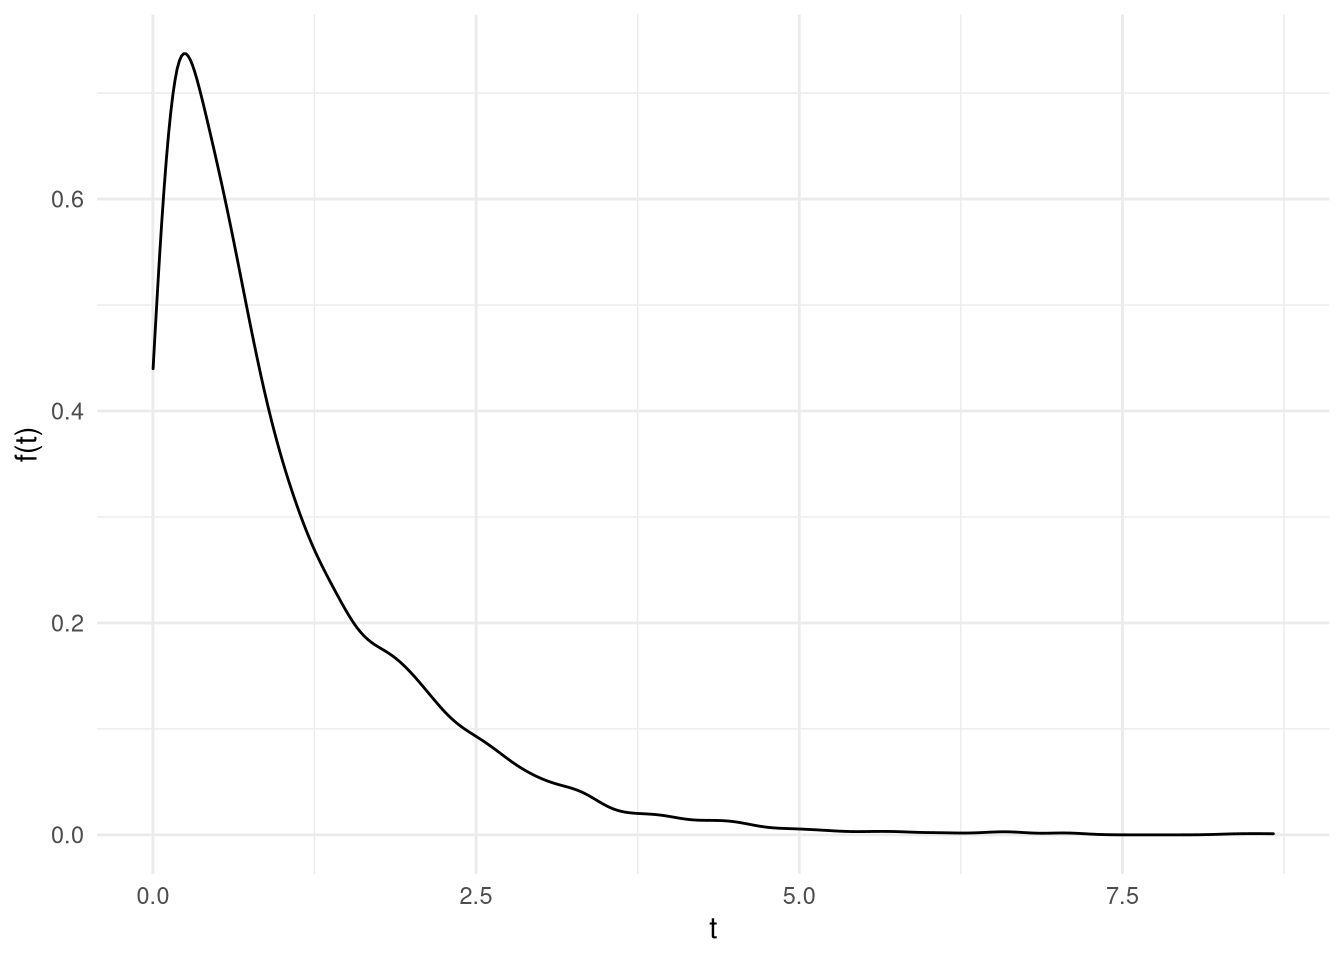
\includegraphics{caps/def_files/figure-pdf/fig-plot-1.pdf}

}

\caption{\label{fig-plot}Exemplo de uma função de densidade}

\end{figure}

Pela Figura~\ref{fig-plot} podemos ter um vislumbre que \(S(0) = 1\) e
\(S(\infty) = 0\).\\
A demonstração de tais fatos fica a cargo do leitor, basta notar que
\(S(t) = 1 - F(t)\) e usar as propriedades da \(F\).

Por consequência a probabilidade de não sobreviver até um certo tempo
\(t\) é: \[
1- S(t)
\] Assim a probabilidade de não sobreviver em um intervalo \((t_1,t_2)\)
é dado por:

\[
1-S(t_2) - (1-S(t_1)) = S(t_1) - S(t_2)
\]

\hypertarget{funuxe7uxe3o-taxa-de-falha}{%
\section{Função taxa de falha}\label{funuxe7uxe3o-taxa-de-falha}}

Fornece o potencial instântaneo do evento \textbf{ocorrer}, dado que o
indivíduo sobreviveu até o tempo \(t\):

\[
\lambda(t)= \dfrac{P(t \leq T < t + \Delta t| T \geq t )}{\Delta t}
\]

Note que estamos interessados em que o evento ocorra, ou seja, em termos
de interpretação é o \textbf{oposto} da função de sobrevivência.

\hypertarget{consequuxeancias}{%
\subsection{Consequências}\label{consequuxeancias}}

\begin{itemize}
\tightlist
\item
  \(\lambda(t) \geq 0\)

  Demonstração

  É trivial pois por definição medidas de probabilidade \(\in [0,1]\) e
  \(\Delta_t \geq 0\) portanto um produto de números positivos
\item
  \(\lambda(t) =\dfrac{f(t)}{S(t)} = -\dfrac{d}{dt}\bigg(log(S(t))\bigg)\)
\end{itemize}

\hypertarget{programando}{%
\chapter{Programando}\label{programando}}

Nessa seção vamos aplicar o conceitos em três linguagens de programação,
a saber: Python e R

\hypertarget{layout-buxe1sico}{%
\section{Layout Básico}\label{layout-buxe1sico}}

Os dados de sobrevivência possuem um layout estabelecido, que é dado a
seguir:

\begin{longtable}[]{@{}llllll@{}}
\toprule()
Id & \(T\) & \(s_i\) & \(X_i\) & \ldots{} & \(X_p\) \\
\midrule()
\endhead
1 & \(t_1\) & \(s_1\) & \(x_{1i}\) & \ldots{} & \(x_{1p}\) \\
2 & \(t_2\) & \(s_2\) & \(x_{2i}\) & \ldots{} & \(x_{2p}\) \\
. & . & . & . & . & . \\
. & . & . & . & . & . \\
n & \(t_n\) & \(s_n\) & \(x_{ni}\) & \ldots{} & \(x_{np}\) \\
\bottomrule()
\end{longtable}

R

\begin{Shaded}
\begin{Highlighting}[]
\NormalTok{tempo }\OtherTok{\textless{}{-}} \FunctionTok{c}\NormalTok{(}\DecValTok{1}\NormalTok{, }\DecValTok{2}\NormalTok{, }\DecValTok{3}\NormalTok{, }\DecValTok{3}\NormalTok{, }\DecValTok{3}\NormalTok{, }\DecValTok{5}\NormalTok{, }\DecValTok{5}\NormalTok{, }\DecValTok{16}\NormalTok{, }\DecValTok{16}\NormalTok{, }\DecValTok{16}\NormalTok{, }\DecValTok{16}\NormalTok{, }\DecValTok{16}\NormalTok{, }\DecValTok{16}\NormalTok{, }\DecValTok{6}\NormalTok{, }\DecValTok{16}\NormalTok{, }\DecValTok{1}\NormalTok{, }\DecValTok{1}\NormalTok{, }\DecValTok{1}\NormalTok{, }\DecValTok{1}\NormalTok{, }\DecValTok{4}\NormalTok{, }\DecValTok{5}\NormalTok{, }\DecValTok{7}\NormalTok{, }\DecValTok{8}\NormalTok{, }\DecValTok{10}\NormalTok{, }\DecValTok{10}\NormalTok{, }\DecValTok{12}\NormalTok{, }\DecValTok{16}\NormalTok{, }\DecValTok{16}\NormalTok{, }\DecValTok{16}\NormalTok{)}
\NormalTok{censura }\OtherTok{\textless{}{-}} \FunctionTok{c}\NormalTok{(}\DecValTok{0}\NormalTok{, }\DecValTok{0}\NormalTok{, }\DecValTok{1}\NormalTok{, }\DecValTok{1}\NormalTok{, }\DecValTok{0}\NormalTok{, }\DecValTok{0}\NormalTok{, }\DecValTok{0}\NormalTok{, }\DecValTok{0}\NormalTok{, }\DecValTok{0}\NormalTok{, }\DecValTok{0}\NormalTok{, }\DecValTok{0}\NormalTok{, }\DecValTok{0}\NormalTok{, }\DecValTok{0}\NormalTok{, }\DecValTok{0}\NormalTok{, }\DecValTok{0}\NormalTok{, }\DecValTok{1}\NormalTok{, }\DecValTok{1}\NormalTok{, }\DecValTok{1}\NormalTok{, }\DecValTok{0}\NormalTok{, }\DecValTok{0}\NormalTok{, }\DecValTok{1}\NormalTok{, }\DecValTok{1}\NormalTok{, }\DecValTok{1}\NormalTok{, }\DecValTok{1}\NormalTok{, }\DecValTok{0}\NormalTok{, }\DecValTok{0}\NormalTok{, }\DecValTok{0}\NormalTok{, }\DecValTok{0}\NormalTok{, }\DecValTok{0}\NormalTok{)}
\NormalTok{grupo }\OtherTok{\textless{}{-}} \FunctionTok{c}\NormalTok{(}\FunctionTok{rep}\NormalTok{(}\DecValTok{1}\NormalTok{, }\DecValTok{15}\NormalTok{), }\FunctionTok{rep}\NormalTok{(}\DecValTok{0}\NormalTok{, }\DecValTok{14}\NormalTok{))}
\NormalTok{dados }\OtherTok{\textless{}{-}}\NormalTok{ tempo  }\SpecialCharTok{|\textgreater{}} 
            \FunctionTok{cbind}\NormalTok{(censura)  }\SpecialCharTok{|\textgreater{}} 
            \FunctionTok{cbind}\NormalTok{(grupo)}
\NormalTok{dados  }\SpecialCharTok{|\textgreater{}} 
        \FunctionTok{head}\NormalTok{()}
\end{Highlighting}
\end{Shaded}

\begin{verbatim}
     tempo censura grupo
[1,]     1       0     1
[2,]     2       0     1
[3,]     3       1     1
[4,]     3       1     1
[5,]     3       0     1
[6,]     5       0     1
\end{verbatim}

Python

\begin{Shaded}
\begin{Highlighting}[]
\ImportTok{import}\NormalTok{ pandas }\ImportTok{as}\NormalTok{ pd}
\ImportTok{import}\NormalTok{ numpy }\ImportTok{as}\NormalTok{ np}

\NormalTok{tempo }\OperatorTok{=}\NormalTok{ [}\DecValTok{1}\NormalTok{, }\DecValTok{2}\NormalTok{, }\DecValTok{3}\NormalTok{, }\DecValTok{3}\NormalTok{, }\DecValTok{3}\NormalTok{, }\DecValTok{5}\NormalTok{, }\DecValTok{5}\NormalTok{, }\DecValTok{16}\NormalTok{, }\DecValTok{16}\NormalTok{, }\DecValTok{16}\NormalTok{, }\DecValTok{16}\NormalTok{, }\DecValTok{16}\NormalTok{, }\DecValTok{16}\NormalTok{, }\DecValTok{16}\NormalTok{, }\DecValTok{16}\NormalTok{, }\DecValTok{1}\NormalTok{, }\DecValTok{1}\NormalTok{, }\DecValTok{1}\NormalTok{, }\DecValTok{1}\NormalTok{, }\DecValTok{4}\NormalTok{, }\DecValTok{5}\NormalTok{, }\DecValTok{7}\NormalTok{, }\DecValTok{8}\NormalTok{, }\DecValTok{10}\NormalTok{, }\DecValTok{10}\NormalTok{, }\DecValTok{12}\NormalTok{, }\DecValTok{16}\NormalTok{, }\DecValTok{16}\NormalTok{, }\DecValTok{16}\NormalTok{]}
\NormalTok{censura }\OperatorTok{=}\NormalTok{ [}\DecValTok{0}\NormalTok{, }\DecValTok{0}\NormalTok{, }\DecValTok{1}\NormalTok{, }\DecValTok{1}\NormalTok{, }\DecValTok{0}\NormalTok{, }\DecValTok{0}\NormalTok{, }\DecValTok{0}\NormalTok{, }\DecValTok{0}\NormalTok{, }\DecValTok{0}\NormalTok{, }\DecValTok{0}\NormalTok{, }\DecValTok{0}\NormalTok{, }\DecValTok{0}\NormalTok{, }\DecValTok{0}\NormalTok{, }\DecValTok{0}\NormalTok{, }\DecValTok{0}\NormalTok{, }\DecValTok{1}\NormalTok{, }\DecValTok{1}\NormalTok{, }\DecValTok{1}\NormalTok{, }\DecValTok{0}\NormalTok{, }\DecValTok{0}\NormalTok{, }\DecValTok{1}\NormalTok{, }\DecValTok{1}\NormalTok{, }\DecValTok{1}\NormalTok{, }\DecValTok{1}\NormalTok{, }\DecValTok{0}\NormalTok{, }\DecValTok{0}\NormalTok{, }\DecValTok{0}\NormalTok{, }\DecValTok{0}\NormalTok{, }\DecValTok{0}\NormalTok{]}
\NormalTok{grupo }\OperatorTok{=}\NormalTok{ np.concatenate((np.repeat(}\DecValTok{1}\NormalTok{, }\DecValTok{15}\NormalTok{), np.repeat(}\DecValTok{0}\NormalTok{, }\DecValTok{14}\NormalTok{)))}

\NormalTok{dados }\OperatorTok{=}\NormalTok{ pd.DataFrame(\{}\StringTok{\textquotesingle{}tempo\textquotesingle{}}\NormalTok{:tempo,}\StringTok{\textquotesingle{}censura\textquotesingle{}}\NormalTok{:censura,}\StringTok{\textquotesingle{}grupo\textquotesingle{}}\NormalTok{:grupo\})}
\NormalTok{dados.head()}
\end{Highlighting}
\end{Shaded}

\begin{verbatim}
   tempo  censura  grupo
0      1        0      1
1      2        0      1
2      3        1      1
3      3        1      1
4      3        0      1
\end{verbatim}

\hypertarget{anuxe1lise-descritiva}{%
\chapter{Análise Descritiva}\label{anuxe1lise-descritiva}}

Em Estatística é bastante usual fazer análise descritiva dos dados, como
medidas resumo, gráficos e tabelas. Aqui também iremos elaborar análise
descritivas, porém com foco nas medidas de sobrevivência e risco.

\begin{tcolorbox}[standard jigsaw,opacityback=0, bottomtitle=1mm, titlerule=0mm, rightrule=.15mm, toprule=.15mm, opacitybacktitle=0.6, title=\textcolor{quarto-callout-note-color}{\faInfo}\hspace{0.5em}{Nota}, arc=.35mm, colbacktitle=quarto-callout-note-color!10!white, bottomrule=.15mm, toptitle=1mm, leftrule=.75mm, left=2mm, colframe=quarto-callout-note-color-frame, coltitle=black, colback=white]
O símbolo \textbf{\#} aqui é utilizado para indicar a cardinalidade
(quantidade de elementos) de um conjunto.

Por exemplo o conjunto \(A = \{a,b,d\}\), possui cardinalidade 3, isso é
\#A \(=3\)
\end{tcolorbox}

\hypertarget{estimando-a-funuxe7uxe3o-de-sobrevivuxeancia}{%
\section{Estimando a função de
sobrevivência}\label{estimando-a-funuxe7uxe3o-de-sobrevivuxeancia}}

Vamos nessa subseção estudar algumas maneiras de estimar a função de
sobrevivência \(S(t)\)

\hypertarget{sem-dados-de-censura}{%
\subsection{Sem dados de censura}\label{sem-dados-de-censura}}

Uma maneira bastante intuitiva para estimarmos \(S(t)\) é tomarmos a
quantidade de indíviduos que não falharam até o tempo \(t\) dividindo
pelo total de indíviduos no estudo \[
\hat{S}(t) = \dfrac{\# \text{Observações que não falharam até t}}{\# \text{Observações}}
\]

Na prática, \(S(t)\) será obtida por algum estimador, e portanto seu
gráfico terá um formato de escada, como dado a seguir:

\begin{figure}

{\centering 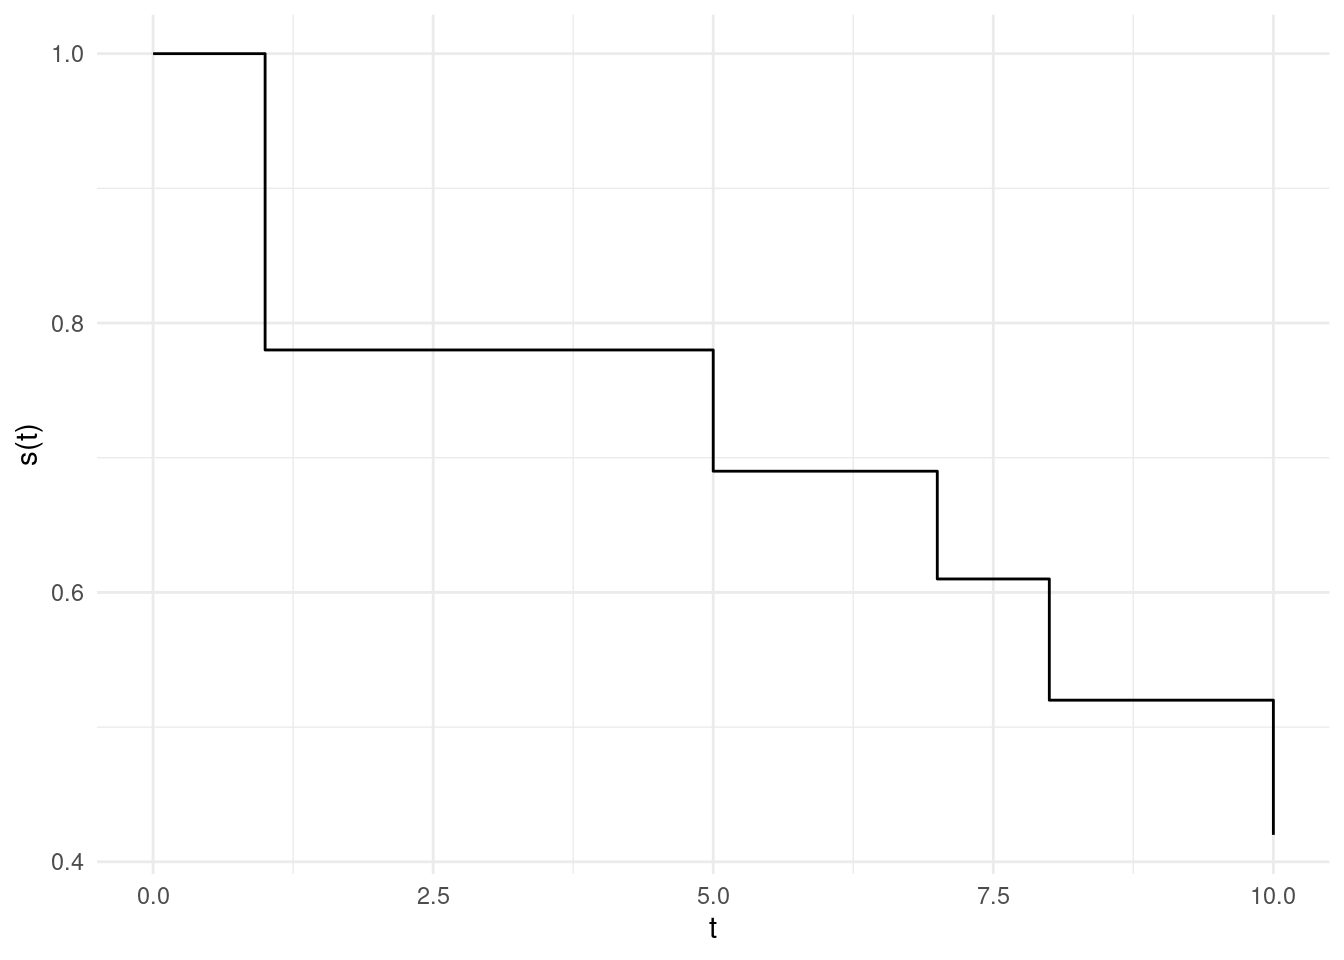
\includegraphics{caps/eda_files/figure-pdf/fig-step-1.pdf}

}

\caption{\label{fig-step}Exemplo de uma função de sobrevivência na
prática}

\end{figure}

Pelo Figura~\ref{fig-step} nota-se que a função mantém-se constante em
alguns intervalos e tem um decaimento em alguns pontos específicos, a
proxima seção formaliza tal ideia.

\hypertarget{estimador-de-kaplan-meier}{%
\chapter{Estimador de Kaplan-Meier}\label{estimador-de-kaplan-meier}}

O estimador de Kaplan-Meier também denominado limite-produto é uma
adaptação da ideia `ingênua' que utilizamos na seção anterior. Ele
fornece uma maneira simples, mas eficiente de estimar a função de
sobrevivência. De forma intuitiva, dividimos o tempo \(t\) em uma série
de intervalos de acordo com os eventos observados ou dados censurados,
após isso calculamos uma sequência de produto de probabilidade
condicionais

\hypertarget{outra-maneira-de-layout-para-os-dados}{%
\section{Outra maneira de layout para os
dados}\label{outra-maneira-de-layout-para-os-dados}}

\begin{longtable}[]{@{}
  >{\raggedright\arraybackslash}p{(\columnwidth - 10\tabcolsep) * \real{0.1290}}
  >{\raggedright\arraybackslash}p{(\columnwidth - 10\tabcolsep) * \real{0.1613}}
  >{\raggedright\arraybackslash}p{(\columnwidth - 10\tabcolsep) * \real{0.2258}}
  >{\raggedright\arraybackslash}p{(\columnwidth - 10\tabcolsep) * \real{0.1613}}
  >{\raggedright\arraybackslash}p{(\columnwidth - 10\tabcolsep) * \real{0.1613}}
  >{\raggedright\arraybackslash}p{(\columnwidth - 10\tabcolsep) * \real{0.1613}}@{}}
\toprule()
\begin{minipage}[b]{\linewidth}\raggedright
t ordenados
\end{minipage} & \begin{minipage}[b]{\linewidth}\raggedright
int
\end{minipage} & \begin{minipage}[b]{\linewidth}\raggedright
\# de falhas
\end{minipage} & \begin{minipage}[b]{\linewidth}\raggedright
\(n_j\)
\end{minipage} & \begin{minipage}[b]{\linewidth}\raggedright
\(m_j\)
\end{minipage} & \begin{minipage}[b]{\linewidth}\raggedright
\end{minipage} \\
\midrule()
\endhead
0 & \([0,t_1)\) & \(0\) & \(k\) & \(m_{1}\) & \\
\(t_1\) & \([t_1,t_2)\) & \(d_2\) & \(k-(d_1+ m_1)\) & \(m_{2}\) & \\
\(t_2\) & \([t_2,t_3)\). & . & . & . & \\
. & . & . & . & . & \\
. & . & . & . & . & \\
k & \([t_{k},t_{k+\epsilon})\) & \(d_k\) & \(k - \sum_i (d_i + m_i)\) &
\(m_{n}\) & \\
\bottomrule()
\end{longtable}

\begin{itemize}
\tightlist
\item
  \textbf{int}: São os intervalos
\item
  \textbf{\# de falhas}: É o número de falhas naquele intervalo
\item
  \textbf{\(n_j\)} : É a quantidade de observações que ainda não
  falharam ou foram censuradas naquele intervalo (as vezes chamado de
  indivíduos sob risco)
\item
  \textbf{\(c_j\)}: Quantidade de censuras naquele intervalo.
\end{itemize}

Assim fica fácil ver que no tempo 0 temos 0 falhas, porque como vamos
ver a seguir a construção dos intervalos começa a partir do primeiro
tempo que acontece um evento, e como temos 0 falhas temos portanto todos
(k) os indivíduos sem o evento de interesse

\hypertarget{formalizando}{%
\section{Formalizando}\label{formalizando}}

Sabemos que \(S(t) = P(T>t)\), vamos supor que já construímos a tabela e
possuímos o tempo 3 e 1, assim queremos calcular, por exemplo:
\[S(3) = P(T>3)\]

Podemos fazer a seguinte manipulação: \[
S(3) = P(T>3) = P(T>1,T>3) = P(T>1)P(T>3|T>1)
\]

\begin{tcolorbox}[standard jigsaw,opacityback=0, bottomtitle=1mm, titlerule=0mm, rightrule=.15mm, toprule=.15mm, opacitybacktitle=0.6, title=\textcolor{quarto-callout-note-color}{\faInfo}\hspace{0.5em}{Nota}, arc=.35mm, colbacktitle=quarto-callout-note-color!10!white, bottomrule=.15mm, toptitle=1mm, leftrule=.75mm, left=2mm, colframe=quarto-callout-note-color-frame, coltitle=black, colback=white]
Lembre que \(f(X|Y) = \dfrac{f(X,Y)}{f(Y)}\)

E que se A é subconjunto de B, então A \(\cap\) B \(=\) A (relacione aos
intervalos \((1,\infty)\) e \((3,\infty)\)
\end{tcolorbox}

Vamos utilizar o seguinte exemplo para ilustrar a ideia anterior:

\begin{longtable}[]{@{}llllll@{}}
\toprule()
t ordenados & int & \# de falhas (\(d_j\)) & \(n_j\) & \(\hat{S}(.)\)
& \\
\midrule()
\endhead
0 & \([0,1)\) & \(0\) & \(14\) & \(1\) & \\
\(1\) & \([1,5)\) & \(3\) & \(14\) & \(0.78\) & \\
\(5\) & \([5,7)\) & \(1\) & \(9\) & . & \\
\(7\) & \([7,8)\) & \(1\) & \(8\) & . & \\
\(8\) & \([8,10)\) & \(1\) & \(7\) & . & \\
\(10\) & \([10,16)\) & \(1\) & \(6\) & \(x_{np}\) & \\
\bottomrule()
\end{longtable}

Para calcular \(\hat{S}(1)\), fazemos então: \[
P(T>1) = P(T>0,T>1) = P(T>0)P(T>1 |T>0)
\] Sabemos que \(P(T>0) = 1\) como comentado anteriormente. Temos 3
acontecimentos do evento de interesse no tempo \(t=1\) e 14 observações
restantes, assim a probabilidade de `falhar' nesse intervalo é
\(\dfrac{3}{14}\), portanto a probabilidade de sobreviver é
\(1 - \dfrac{3}{14}\), substituindo as informações tem-se portanto que
\(\hat{S}(1) = 0.786\)

Para \(\hat{S}(5)\), fazemos a mesma decomposição de probabilidade e
chegamos em:

\[
\hat{S}(5) =  P(T>1)P(T>5|T>1)
\] Como calculado anteriormente \(P(T>1) = 1-\dfrac{3}{14}\) e
\(P(T>5|T>1) = 1 - \dfrac{1}{9}\).

Fica claro então a relação de recursão, pois para o cálculo da
estimativa utiliza-se todas as probabilidades calculadas anteriormente,
generalizando temos:

\[
S(t_j) =(1-q_1)(1-q_2)...(1-q_j) =  \prod_{j:t_j<t} \bigg(1 - \dfrac{d_j}{n_j}\bigg) = \prod_{j:t_j<t} \bigg(\dfrac{n_j - d_j}{n_j}\bigg)
\]

Onde \(q_j\) é a probabilidade de uma observação ter o evento de
interesse no intervalo \([t_{j-1},t_j)\) sabendo-se que não teve em
\(t_{j-1}\), formalizando tem-se:

\[
q_j = P(T \in [t_{j-1},t_j)] | T> t_{j-1}) 
\]

Assim o estimador reduz-se a estimar os \(q_j\), reescrevendo usando
alguns termos já citados temos:

\[
\hat{q}_j = \dfrac{\# \quad \text{de falhas em} \quad t_j}{\# \quad  \text{Observações sobre risco}}
\]

\begin{tcolorbox}[standard jigsaw,opacityback=0, bottomtitle=1mm, titlerule=0mm, rightrule=.15mm, toprule=.15mm, opacitybacktitle=0.6, title=\textcolor{quarto-callout-important-color}{\faExclamation}\hspace{0.5em}{Importante}, arc=.35mm, colbacktitle=quarto-callout-important-color!10!white, bottomrule=.15mm, toptitle=1mm, leftrule=.75mm, left=2mm, colframe=quarto-callout-important-color-frame, coltitle=black, colback=white]
Os métodos construídos anteriormente são ditos
\textbf{não-paramétricos}, pois para a derivação dos estimadores não se
faz pressuposto de distribuição para a variável aleatória \(T\)
\end{tcolorbox}

\hypertarget{propriedades-do-estimador}{%
\section{Propriedades do estimador}\label{propriedades-do-estimador}}

Como temos um estimador pontual, podemos também construir intervalos de
confiança para a estimativas.

\hypertarget{variuxe2ncia-do-estimador}{%
\subsection{Variância do Estimador}\label{variuxe2ncia-do-estimador}}

Ora ora, para calcular a variância do estimador precisamos saber a
distribuição do estimador, então aqui vamos nos conter com o estimador
da variância do estimador, que é dado por: \[
\widehat{\text{Var}}(\hat{S}(t)) = [\hat{S}(t)]^{2}\sum_{j:t_j<t}\dfrac{d_j}{n_j(n_j - d_j)} 
\]

\hypertarget{cuxf3digos}{%
\section{Códigos}\label{cuxf3digos}}

Python

\begin{Shaded}
\begin{Highlighting}[]
\ImportTok{import}\NormalTok{ pandas }\ImportTok{as}\NormalTok{ pd}
\ImportTok{import}\NormalTok{ numpy }\ImportTok{as}\NormalTok{ np}
\ImportTok{from}\NormalTok{ lifelines }\ImportTok{import}\NormalTok{ KaplanMeierFitter}
\CommentTok{\#\%\% }
\NormalTok{tempo }\OperatorTok{=}\NormalTok{ [}\DecValTok{1}\NormalTok{, }\DecValTok{1}\NormalTok{, }\DecValTok{1}\NormalTok{, }\DecValTok{1}\NormalTok{, }\DecValTok{4}\NormalTok{, }\DecValTok{5}\NormalTok{, }\DecValTok{7}\NormalTok{, }\DecValTok{8}\NormalTok{, }\DecValTok{10}\NormalTok{, }\DecValTok{10}\NormalTok{, }\DecValTok{12}\NormalTok{, }\DecValTok{16}\NormalTok{, }\DecValTok{16}\NormalTok{, }\DecValTok{16}\NormalTok{]}
\NormalTok{falha }\OperatorTok{=}\NormalTok{ [}\DecValTok{1}\NormalTok{, }\DecValTok{1}\NormalTok{, }\DecValTok{1}\NormalTok{, }\DecValTok{0}\NormalTok{, }\DecValTok{0}\NormalTok{, }\DecValTok{1}\NormalTok{, }\DecValTok{1}\NormalTok{, }\DecValTok{1}\NormalTok{, }\DecValTok{1}\NormalTok{, }\DecValTok{0}\NormalTok{, }\DecValTok{0}\NormalTok{, }\DecValTok{0}\NormalTok{, }\DecValTok{0}\NormalTok{, }\DecValTok{0}\NormalTok{]}

\NormalTok{dados }\OperatorTok{=}\NormalTok{ pd.DataFrame(\{}\StringTok{\textquotesingle{}tempo\textquotesingle{}}\NormalTok{:tempo,}\StringTok{\textquotesingle{}censura\textquotesingle{}}\NormalTok{:falha\})}

\CommentTok{\#\%\%}
\NormalTok{KaplanMeierFitter().fit(dados[}\StringTok{\textquotesingle{}tempo\textquotesingle{}}\NormalTok{],dados[}\StringTok{\textquotesingle{}censura\textquotesingle{}}\NormalTok{]).survival\_function\_}
\end{Highlighting}
\end{Shaded}

\begin{verbatim}
          KM_estimate
timeline             
0.0          1.000000
1.0          0.785714
4.0          0.785714
5.0          0.698413
7.0          0.611111
8.0          0.523810
10.0         0.436508
12.0         0.436508
16.0         0.436508
\end{verbatim}

\hypertarget{summary}{%
\chapter{Summary}\label{summary}}

In summary, this book has no content whatsoever.

\hypertarget{referuxeancias}{%
\chapter*{Referências}\label{referuxeancias}}
\addcontentsline{toc}{chapter}{Referências}

\hypertarget{refs}{}
\begin{CSLReferences}{1}{0}
\leavevmode\vadjust pre{\hypertarget{ref-colosimo2006analise}{}}%
Colosimo, Suely Ruiz, Enrico Antonio e Giolo. 2006. \emph{An{á}lise de
sobreviv{ê}ncia aplicada}. Editora Blucher.

\end{CSLReferences}

\end{document}
